\section{Hip\'otesis de interacciones esenciales~\citep{he2006}}
Como hemos mostrado en la secci\'on \ref{sec:jeong} la correlaci\'on vista por Jeong es corroborada, sin embargo su hip\'otesis
de esencialidad debido centralidad por grado no responde al comportamiento real de las redes. He y sus colegas plantean una
hip\'otesis alternativa: La esencialidad se debe a la participaci\'on en interacciones esenciales y no esencialidad 
\textit{unitaria} como pensaba Jeong. Bajo esta hip\'otesis la regla de Centralidad-Letalidad se explica debido a que 
los hubs, al tener mayor cantidad de interacciones, tienen mayor probabilidad de pertenecer a una interacci\'on esencial.

El modelo de He considera dos condiciones de esencialidad: La prote\'ina participa en una interacci\'on esencial representada
en la red con una probabilidad $\alpha$ \'o la prote\'ina es esencial debido a alg\'un otro factor que la red no es capaz de
mostrar. As\'i la probabilidad de que un nodo de grado $k$ no participe en una interacc\'ion esencial es 
$(1-\alpha)(1-\alpha)\cdots(1-\alpha) = (1-\alpha)^k$ y la probabilidad de no ser esencial debido a otra raz\'on es $(1-\beta)$.
Luego, la probabilidad de no ser esencial es

\begin{align}
    \label{eq:ne}
    1-P_E(k) &= (1-\beta)(1-\alpha)^k\\
    \intertext{finalmente, la probabilidad de esencialidad es}
    P_E(k) &= 1 - (1-\beta)(1-\alpha)^k
\end{align}


A continuaci\'on evaluaremos la calidad de esta hip\'otesis a trav\'es de estimaciones de las probabilidades por dos m\'etodos 
descritos en el trabajo de He y colegas. Cabe se\~nalar que, para lo que resta del an\'alisis, la red AP-MS no ser\'a considerada,
debido a que \citet{he2006} hace referencia redes construidas a partir de asociaci\'on de complejos proteicos podr\'ian 
presentar comportamientos an\'omalos.

\subsection{M\'etodo de Ajuste}
Tomando el logaritmo a la ec. \ref{eq:ne} se tiene 
\begin{align}
    \ln(1-P_E(k)) &= k \ln(1-\alpha) + \ln(1-\beta)
\end{align}
es decir, una relaci\'on lineal entre el grado y la probabilidad de no-esencialidad. \citet{he2006} mensiona que, debido a que
a mayor grado $k$ es m\'as dificil encontrar nodos con grado $k$, por lo que para sus an\'alisis utiliza un umbral superior de
$k=10$. En este trabajo se ha considerado lo mismo. La figura \ref{fig:fit} muestra los resultados del ajuste lineal para 
nuestras redes. Debido al comportamineto irregular de la red Y2H (ver figura \ref{fig:y2h}) esta fue excluida del an\'alisis.

\begin{figure}[!ht]
    \centering
    \begin{subfigure}[b]{0.4\columnwidth}
        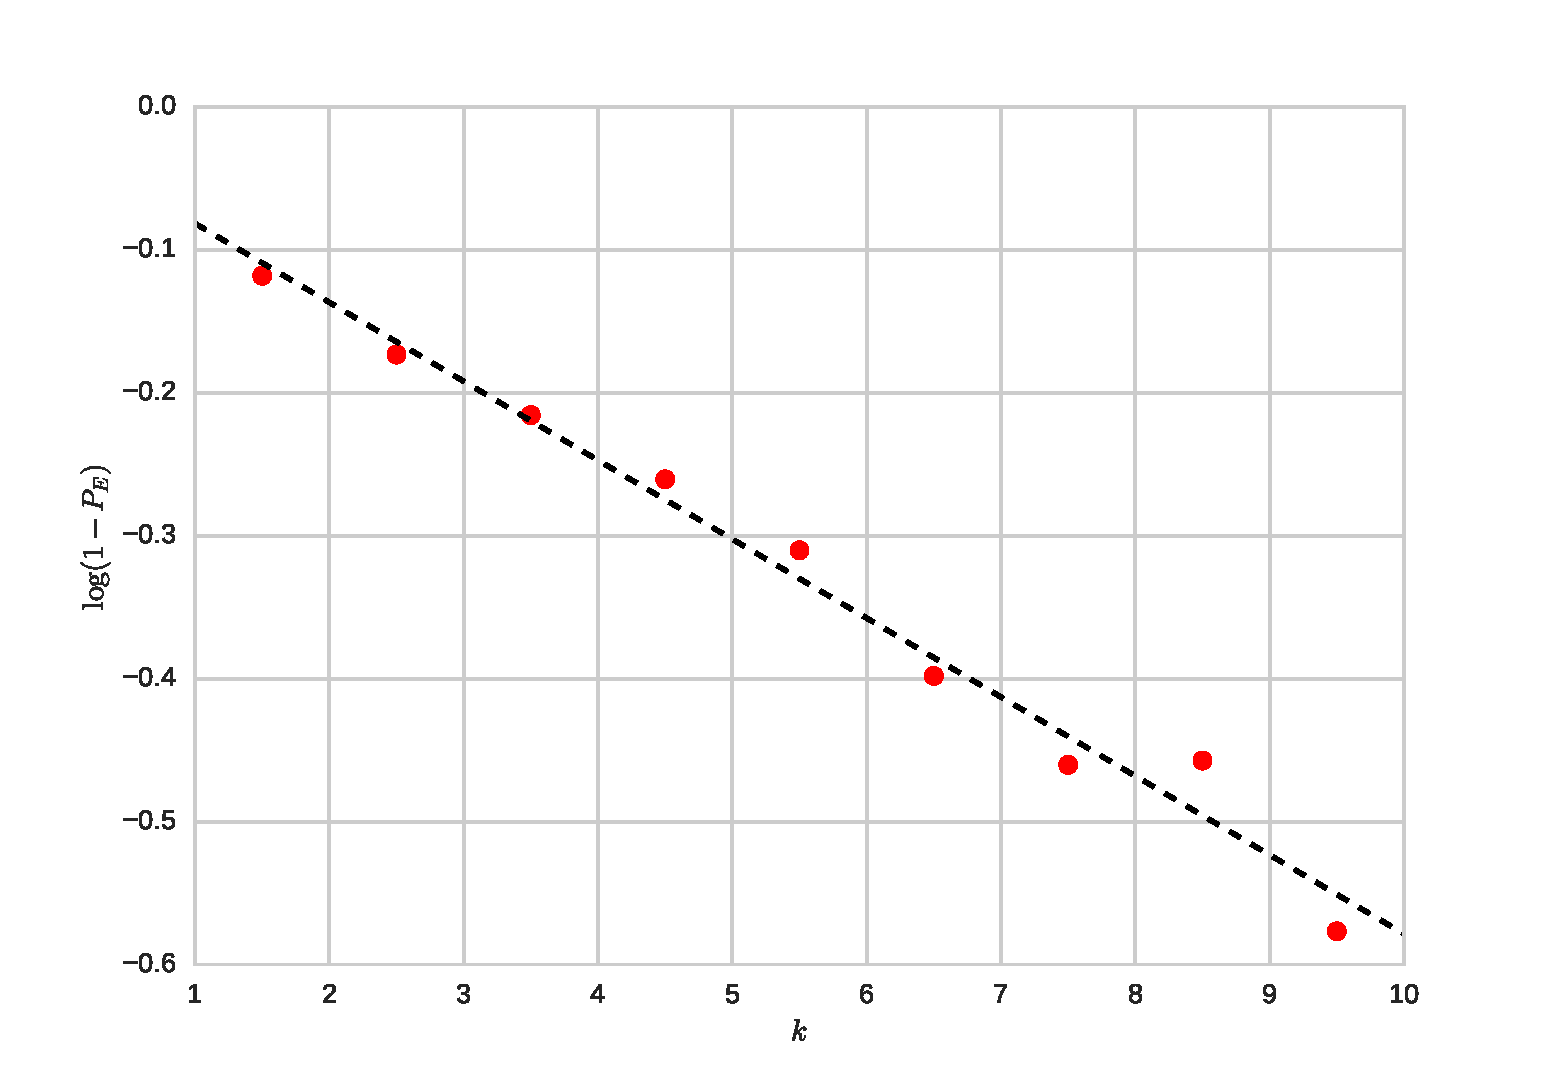
\includegraphics[width=\textwidth]{./schemes/yeast_LIT_Reguly.pdf}
        \caption{\label{fig:LITR}LIT\_Reguly}
    \end{subfigure}
    \begin{subfigure}[b]{0.4\columnwidth}
        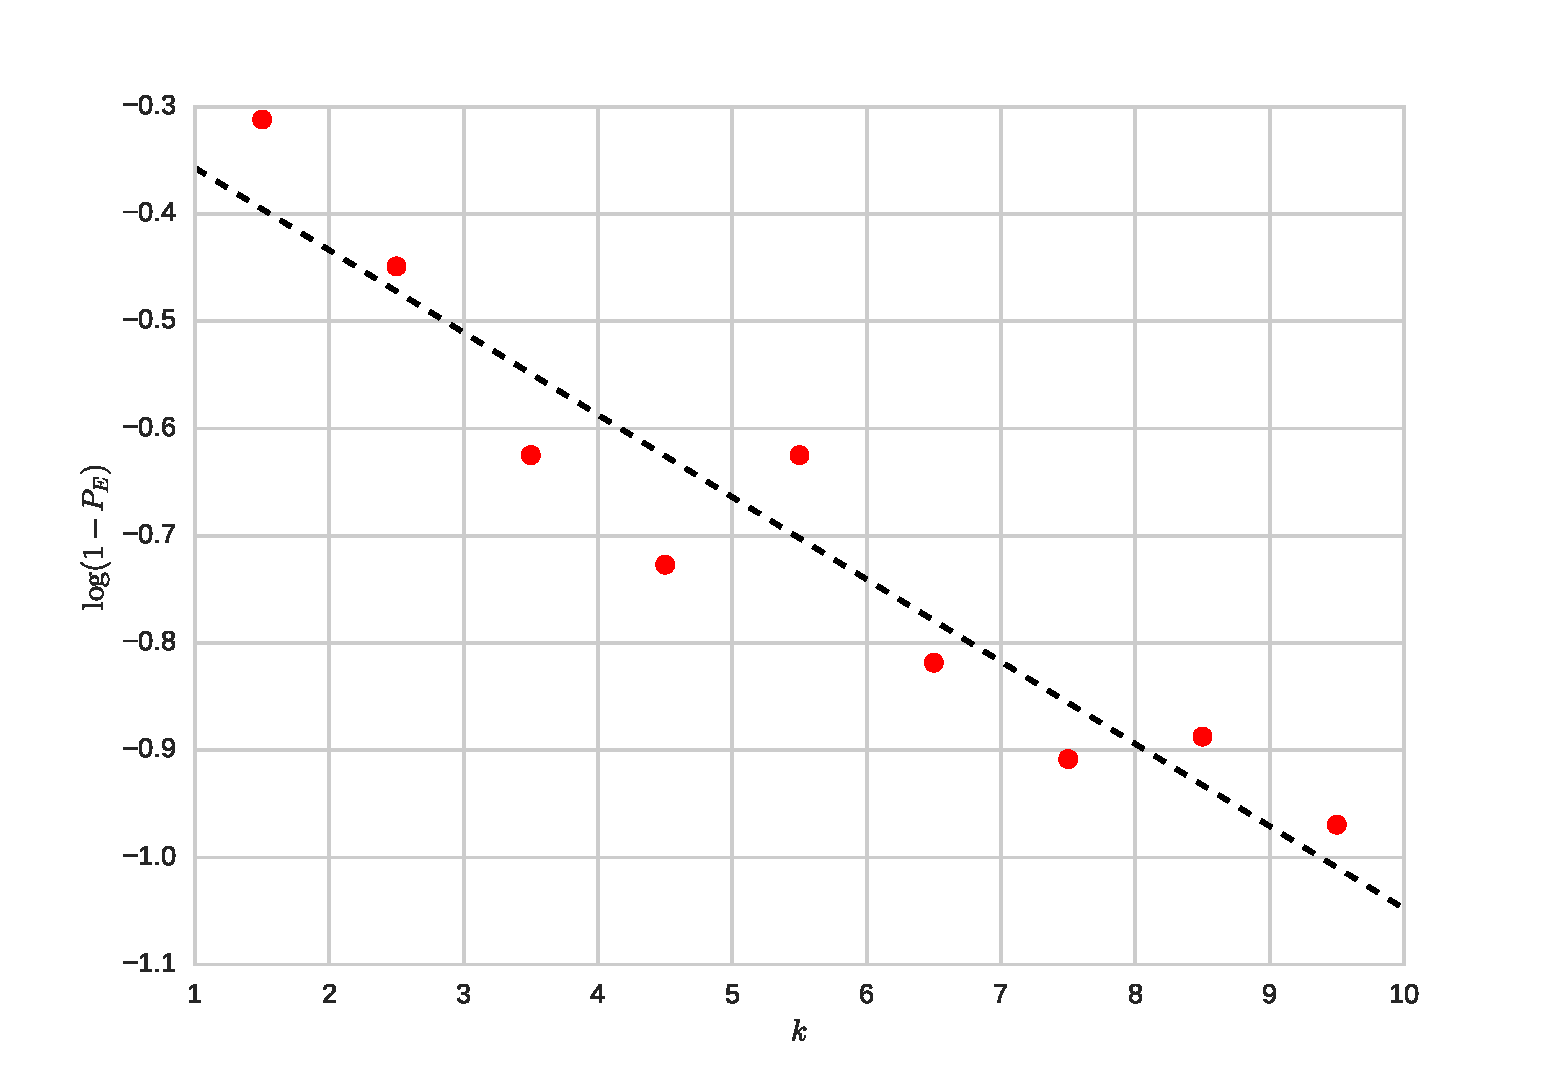
\includegraphics[width=\textwidth]{./schemes/yeast_LIT.pdf}
        \caption{\label{fig:LIT} LIT}
    \end{subfigure}
    \\
    \begin{subfigure}[b]{0.4\columnwidth}
        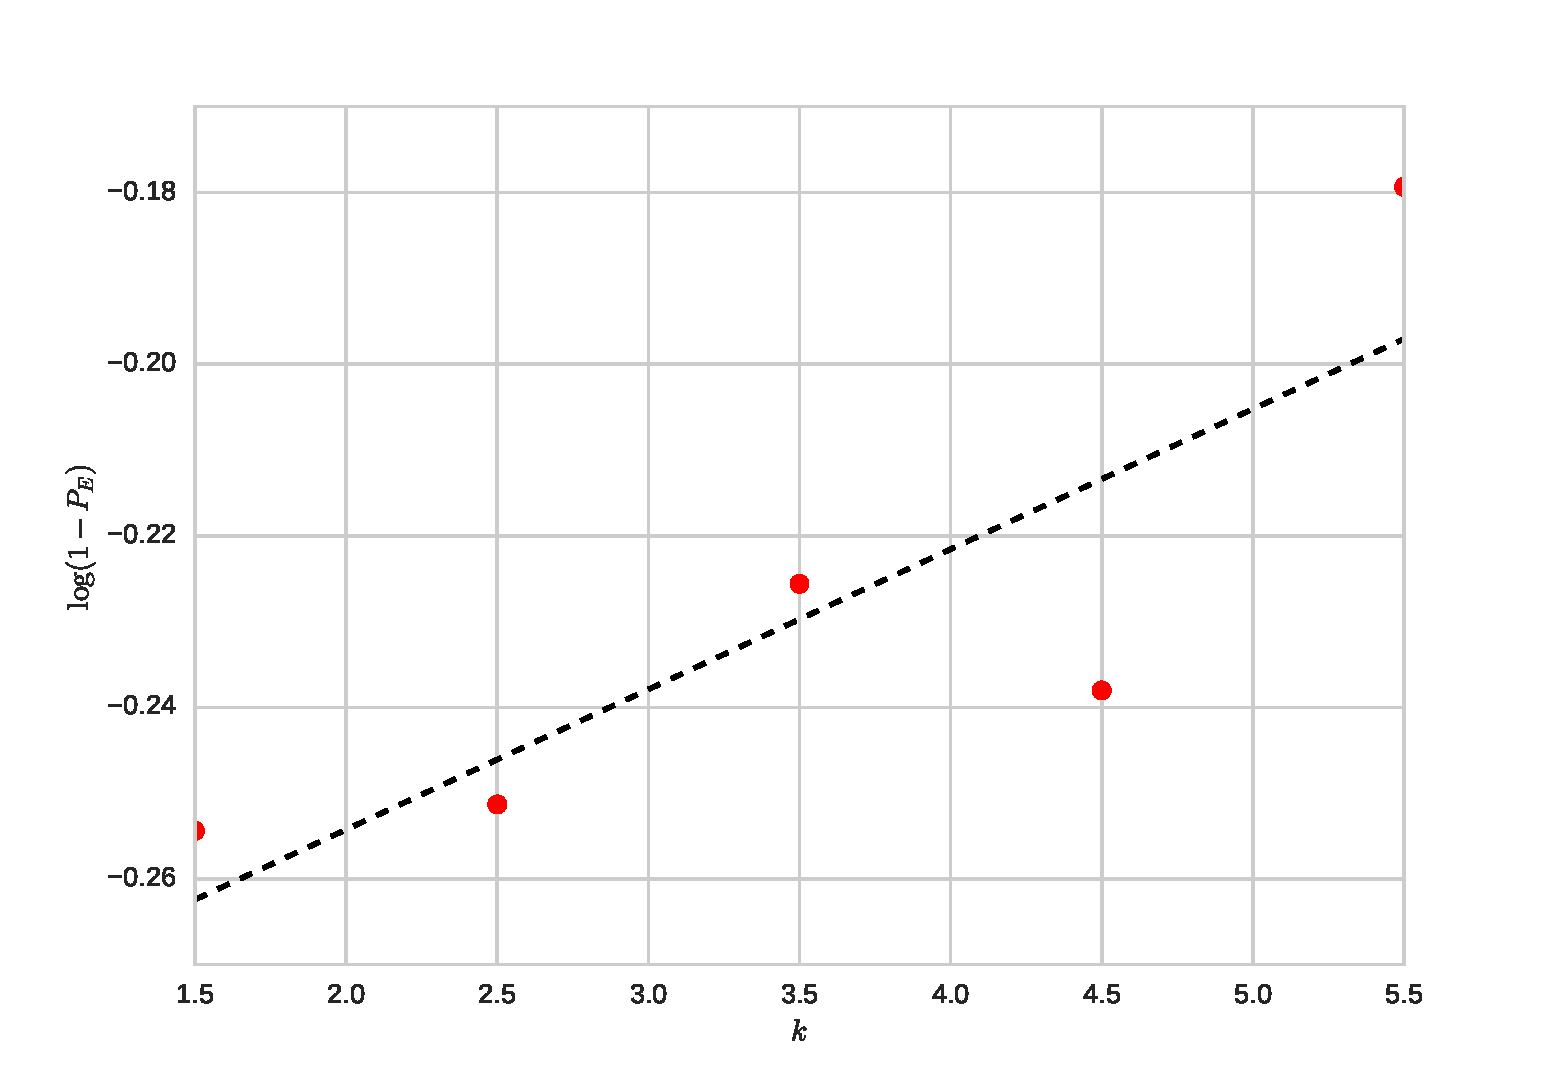
\includegraphics[width=\textwidth]{./schemes/yeast_Y2H.pdf}
        \caption{\label{fig:y2h} Y2H}
    \end{subfigure}
    \caption{\label{fig:fit} Ajustes lineales de las probabilidades de no-esencialidad y grado (ver ec. \ref{eq:ne}. 
    (a) $\alpha = 0.53 \pm 0.002 $ y $\beta = 0.26 \pm 0.017$; (b) $\alpha = 0.073 \pm 0.008$ y $\beta = 0.224 \pm 0.043$. 
    Debido al comportamiento irregular, Y2H ha sido excluida del an\'alisis.}
\end{figure}



\subsection{M\'etodo de simulaciones}
\label{sec:simulacion}

Es dif\'icil identificar interacciones esenciales (PPIs) experimentalmente en la escala gen\'omica, dado que esta identificaci\'on requiere la demostraci\'on de que romper el enlace entre prote\'inas esenciales sin afectar otros aspectos de las funciones prote\'icas causa letalidad o infertilidad.

Aqu\'i usamos un m\'etodo computacional para evaluar la prevalecencia de enlaces esenciales PPIs y la contribuci\'on de PPIs esenciales a la esencialidad de genes al nivel gen\'omico.

Nuestro an\'alisis se enfoca en las redes {\it LIT} y {\it Y2H}.
%, excluyendo a la red {\it AP-MS}, como se hizo en la secci\'on anterior. 
%Tambi\'en excluimos a la red {\it LIT-Reguly} debido 

Como se mencion\'o antes, dos prote\'inas que forman un enlace esencial PPI deben ser esenciales.
Por el contrario, las interacciones entre prote\'inas esenciales (IBEPs, {\it Interaction Between Essential Proteins}, por sus siglas en ingl\'es) pueden o no ser esenciales, dado que la esencialidad de una prote\'ina puede deberse a otros factores adem\'as de las PPIs.
Esta caracter\'istica nos permite estimar el n\'umero de PPIs esenciales en una red, dado queque el n\'umero de IBEPs crece con el n\'umero de PPIs esenciales.

Dado el n\'umero total de interacciones IBEPs $N_{ie}$ para cada red, generamos una red de control haciendo un recableado de los enlaces, manteniendo la distribuci\'on de grado $P(k)$ para cada nodo.
Repitiendo este procedimiento 5000 veces (1000 para la red {\it Y2H}), obtenemos la distribuci\'on del n\'umero ($n_{ie}$) de enlaces esenciales (IBEPs) en redes recableadas al azar.
En todos los caso, el m\'aximo valores de la distribuci\'on no supera el caso de la red real; es decir, $max(n_{ie}) < N_{ie}$ siempre.
Este exceso del caso real tambi\'en se observa en otros casos de PPIs de levadura y en PPIs de nematodos {\bf CITAR 14 y 15, ver p. 2}.

Siguiendo el m\'etodo de \cite{he2006}, determinamos la fracci\'on de interacciones esenciales PPI como $\alpha = (N_{ie} - <n_{ie}>)/(N_{nod})$, siendo $N_{tot}$ el n\'umero total de nodos de la red.
Los valores para las diferentes redes se muestran en la tabla \ref{tab:probas}.


%--- overlapping
% NOTE: sacado de:
% ./beta -- ...
Notar que algunos nodos resultaron afectados por ambos factores; es decir por asignaci\'on random y por PPIs esenciales. 
En particular, para el caso {\it Y2H} es del $22 \pm 6$ \%, y para {\it LIT} es del $7.10 \pm 3.04$.

\begin{figure}
\centering
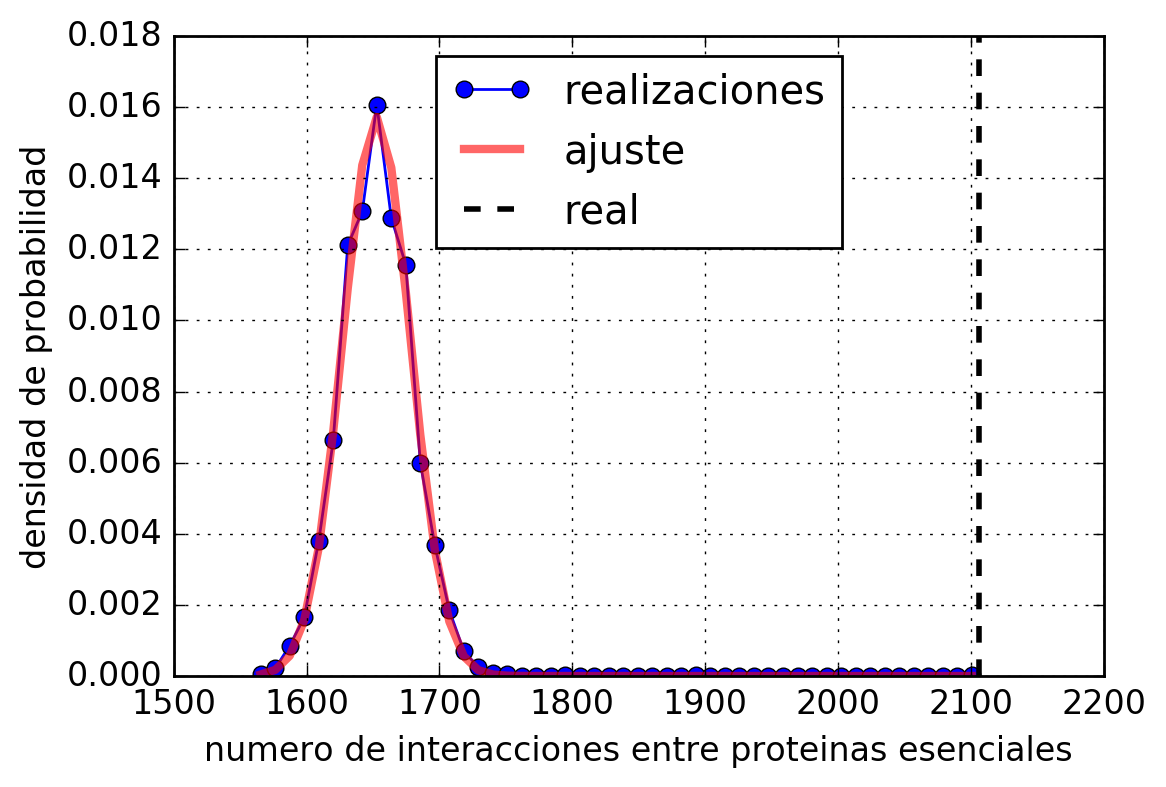
\includegraphics[scale = 0.6]{figuras/hist_LIT} 
\includegraphics[scale = 0.6]{figuras/hist_Y2H} \\
\caption{Distribuciones observadas del n\'umero de interacciones esenciales para los casos random de la redes estudiadas mediante simulaciones, para investigar las probabilidad $\alpha$ y $\beta$ de la red.}
\label{fig:remocion_alternativo}
\end{figure}

%EO



\subsection{Discuci\'on}
\begin{table}[!ht]
    \centering
    \caption{\label{tab:probas} Resumen de probabilidades estimadas para cada red a trav\'es de m\'etodo de ajuste
y simulaciones.}
    {\scriptsize
    \begin{tabularx}{.9\columnwidth}{XlccXccX}
        \hline\hline
        &               &  \multicolumn{2}{c}{Simulaci\'on}  &&  \multicolumn{2}{c}{Ajuste}          &      \\
        \cline{3-4} \cline{6-7}
        &               &   $\alpha$    & $\beta$            &&   $\alpha$       &       $\beta$     & \\
        \hline
        & LIT\_Reguly   &    &         && 0.053$ \pm$ 0.002  & 0.026 $\pm$ 0.017       &               \\
        & LIT           &    &         && 0.073 $\pm$ 0.008  & 0.244 $\pm$ 0.043       &               \\
        & Y2H           &    &         &&    ---             &   ---              &               \\
        \hline\hline
    \end{tabularx}
    }
\end{table}


\begin{table}[!ht]
    \centering
    \caption{\label{tab:pairs} Cantidad de pares totales o de igual caracteristica (ambos esenciales o ambos no esenciale)
    en comparaci\'on al valor estimado desprendido de la hipotesis de \citet{he2006}.}
    {\scriptsize
    \begin{tabularx}{.9\columnwidth}{XlccccX}
        \hline\hline
        &               & Pares   & Pares del   & \multicolumn{2}{c}{Pares esperados del mismo tipo }             \\ 
        \cline{5-6}
        &               & Totales & mismo tipo  & Simulaci\'on  &        Ajuste         &      \\
        \hline
 %       & AP-MS         & 11613 & 5924 & &  &            \\ 
        & LIT\_Reguly   & 10777   & 6187        &               &         5716          &               \\
        & LIT           & 1858    & 1059        &               &          963          &               \\
        & Y2H           & 2258    & 1493        &               &                       &               \\
        \hline\hline
    \end{tabularx}
    }
\end{table}
